\documentclass[12pt]{article}
\usepackage{fullpage,enumitem,amsmath,amssymb,graphicx, listings,cite}%,hyperref}

\usepackage{hyperref}
\usepackage{xcolor}
\hypersetup{
   colorlinks,
   linkcolor={red!50!black},
   citecolor={blue!50!black},
   urlcolor={blue!80!black}
}

\title{Enabling Affordable Precision Agriculture by Sensing Soil Moisture Wirelessly}
\author{Colleen Josephson\\Advised by:  Ranveer Chandra (Microsoft) and Sachin Katti (Stanford)\\\textbf{Do not forward}}

\begin{document}
\maketitle

\begin{abstract}
  The term ``precision agriculture'' has been around since the 1980s,
  and it describes a farming technique that uses extensive measurement
  of crop data to make informed decisions about watering,
  fertilization and more. Despite decades of work, precision
  agriculture is still not widely implemented on working farms. This
  is because the data is hard to collect and process, primarily due to
  the lack of high speed internet access in rural areas, and the high
  cost and difficulty of deploying dense sensor networks. Recent work
  such as Farmbeats~\cite{farmbeats} has made good progress in
  addressing the issues of internet access, but the cost and
  deployability of sensors remains an issue. We seek to address this
  by designing a low-cost and easy-to-use wireless soil moisture
  sensor.
\end{abstract}


\section*{Introduction}

Agriculture is the single largest pressure on the world's sources of
fresh water--- 69\% of the global fresh water supply is used for
agriculture~\cite{water}. Paired with the fact that the world's
population is projected to exceed 9 billion by 2050~\cite{population},
with most of the growth coming from developing nations in Africa,
conservation of fresh water and sufficient food production are key
concerns that need to be addressed. Soil moisture is the most
important measurement for ensuring the maximization of crop yield
without water waste.

Multiple studies show that soil moisture sensors lead to a water
savings of at least 20\%\cite{watersavings}, and in some cases more
than 50\%, while maintaining crop yields. Yet soil sensors are still
not widely deployed on working farms, despite decades of research
confirming the benefits. The lack of widespread adoption can be
attributed to a few key challenges: 1.) high sensor cost 2.)
difficulty of deploying and maintaining the sensors and 3.) difficulty
collecting and processing the sensor data.

The average commercial\footnote{People are often misled by the
  SparkFun soil moisture sensor retailing for \$6.95. This is just a
  raw sensor probe, with no wiring, weatherproofing, testing or
  calibration. The added cost of a power source, data logger and
  wiring is more than \$40, and the system is still not weatherproofed
  or calibrated.} soil moisture sensor is more than \$100, which does
not include the power source or data logger to record and/or transmit
the measurement samples. The cost is at least \$50 to add the cheapest
DIY weatherproof logger and transmitter.  Since soil is not uniform
across a field, nevermind an entire farm, multiple sensors are needed
to accurately measure moisture for irrigation purposes. The average
farm in the United States is 444 acres~\cite{farmsize}. The water cost
for a tomato farm of that size would be approximately \$55,000 per
year~\cite{agwater}~\cite{tomatoes}, which means a precision soil
moisture system would lead to \$11,000 in savings. However, the cost
of deploying 20 sensors~\cite{sensorDensity} per acre would more than
\$1,000,000 with today's sensor costs. The current high cost of
sensors makes it difficult to for the average farmer to justify
investing in precision agriculture. Furthermore, this cost makes soil
moisture sensing completely infeasible for small-holder farmers in
developing nations, which is where the most of the food and water
insecurity will be located.

On top of the high cost, current sensors are not simple to deploy and
maintain. Very few sellers offer a product that includes the sensor,
logger and power source ready for immediate use. Therefore some amount
of setup labor is required for each sensor. Figure 1 shows a typical
sensor and data logging system. Though the sensor is waterproof, the
data logger (in this case an Arduino) needs to be waterproofed and
powered. The soil moisture sensor needs to be burried, which requires
digging a hole to the desired depth. This project also attaches solar
panel to the battery pack, which requires mounting high enough to
harvest sunlight, probably requiring a wooden or metal post. The
laborious process of burying the sensor and mounting the solar panel
would need to be repated for every sensor node on the
farm. Furthermore, the excess cables and bulky box also make the
system easy to tangle in farm eqipment and tools. The sensor system
would need to gently removed and re-deployed every time the field is
tilled. This all adds up to a significant amount of manual labor to
deploy and maintain the soil moisture sensors.

\begin{figure*}[h!]
  \centering
  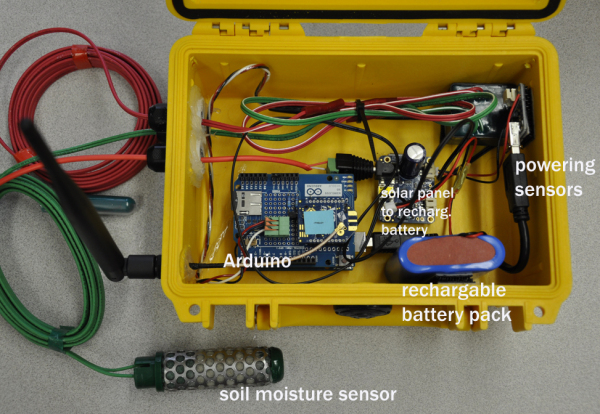
\includegraphics[scale=0.75]{soil_moisture_sn_setup.jpg}\\
  \caption{A weatherproofed soil moisture sensor box from the
    Geosensor Networks Lab~\cite{sensorbox}}
\end{figure*}

Finally, the data needs to be collected from the logger. For a 444
acre farm, the most practical method is wireless collection. Extending
wireless coverage to a large farm is not simple, especially because
cellular coverage in rural areas tends to be poor. A number of recent
works have considered the issue of networking sensors in rural
environments. For example, the 2015 Farmbeats project looks at the
issue of sensor data collection and network access extensively, using
TV whitespace technology to provide a wireless gateway from the field
to the Inernet. Though solving this challenge is also important, the
focus of our research will be on reducing the cost and improving the
deployability and maintainability of soil moisture sensors.

In the next section we will give an overview of current sensing
technology and related work.
    
\section*{Overview of sensing techniques}

The most accurate way to measure soil moisture is gravimetrically,
where a soil sample is taken, weighed, allowed to dry (by oven or
otherwise) and re-weighed~\cite{Noborio2001}. This process is
time-intensive and requires phsyical removal of soil at the depth you
wish to measure, so it is impractical for irrigation purposes. There
are three primary types of practical soil moisture sensors used in
agriculture: tensiometers, resistive sensors, and volumetric
sensors~\cite{sensorTypes}.

\subsubsection*{Tensiometers} Tensiometers measure soil water
tension. An air-free tube of water is attached to a porus tip, such as
ceramic. As water extracted from the soil by plants, the vacuum in the
tube increases. When the soil is irrigated, the pressure decreases. A
pressure sensor at the top of the tube is used to make the moisture
measurements. The response time to moisture changes is typically 2-3
hours. Tensiometers are slightly cheaper than the volumetric sensors
discussed earlier, but still require a dedicated data
logger/transmitter. They typcally require regular maintenance, such as
adding water or removing air from the tube. Tensiometers also only
operate when soils are relatively wet, and cannot be used when there
is any risk of freezing temperatures.

\subsubsection*{Resistive sensors}
Resistive sensors are among the cheapest sensors. These sensors have
two probes in the soil and current passes through the soil between the
probes. The moisture value is determined by measuring the
resistance. DIY soil moisture kits, like the SparkFun~\cite{sparkfun}
sensor, are usually resistive. Resistance-based sensors are the least
accurate, and the probes corrode quickly~\cite{capVSres}. Granular
Granular matrix sensors (GMS) are a variation on resistive
sensors. They measure electrical resistance in a porous medium like
ceramic. As water seeps into the porus medium, it reduces the
electrical resistance. The ceramic in GMSes prevents probe decay and
naturally filter out ions from fertilizer and salt, which improves the
accuracy of the readings. GMSes cost similar to tensiometers, but take
longer to respond, do not work well in very wet soil, and are more
difficult to install. They do, however, require significantly less
maintenance.

\subsubsection*{Volumetric sensors}Volumetric sensors estimate
$\frac{V_{water}}{V_{wet soil}}$, the ratio of the volume of the water
to the volume of the soil plus the same volume of water. As the
volumetric water content changes, the dilectric permittivity constant
of the soil changes. Recall that dielectric permittivity,
$\varepsilon$, is the ability of a substance to hold an electrical
charge. The dielectric permittivty constant (also known as relative
permittivity), $\varepsilon_r$, is the ratio of the permittivity of
the stubstance to the permittivity of free space,
$\varepsilon_0$. Permittivity is often treated as a complex number:
$\varepsilon = \varepsilon' + j\varepsilon ''$, where $\varepsilon '$
is the real component and $\varepsilon''$ is the complex.

There are two main types of volumetric sensors: capacitive and time
domain refelectometry (TDR). Capacitive sensors measure the charge
time of a capacitor, which is a roughly linear function of
$\varepsilon$~\cite{sensorOverview}. Capacative sensors are much less
prone to corrosion than resistive sensors, and are more accurate. For
this reason, capacative sensors are available as commercial-grade soil
moisture sensors. 

Time domain reflectometry (TDR) is another common method for measuring
soil moisture that takes advantage of the frequency dependence of the
dielectric permittivity. It measures the propagation time of EM waves
by sending a pulse down a cable and into the soil probe and measuring
how long it takes before the signal is reflected and returns. This is
known as the \emph{time of flight}, or ToF. This method of soil moisture
measurement is very accurate, but the cheapest sensors are nearly
\$1000 because they require generating wideband signals.

A related technique uses ground penetrating radar (GPR) to calculate
the time of flight. GPR is also wideband and costs thousands of
dollars. Generally the equipment is large (~the size of a lawnmower)
and needs to be dragged across the surface of the soil. This is a
labor intensive process which may not always be possible in dense
crops. Non-contact GPRs exist that can be attached to drones, but
these have lower resolution and can only relaibly measure to a depth
of about 10cm~\cite{gpr}.

\subsubsection*{Novel soil moisture sensors}
A number of recent efforts have explored ways to lower the cost of
soil moisture sensors. \cite{Hasan2013} and uses passive RFID tags to sense
impedance changes caused by soil moisture, but their system requires a
\$1000+ RFID reader, a free-air reference tag, and a delicate antenna
needs to remain on the surface of the soil in order to collect the
readings. \cite{Dey2016} measures the shift in resonance frequency of the
scattering parameter (S-parameter). Their technique required the use
of a vector network analyzer (VNA), so it would require a poentially
costly custom reader. Both of the above approaches were only tested in
an indoors laboratory environment, and they do not provide any
comparisons to the 'ground truth' or an existing commercial sensor.

\cite{Daskalakis2016} attaches a capacative sensor to an above-ground dipole
antenna. The readings are collected using alow-cost software defined
reader. The authors claim a cost of 6 Euro, which is the lowest-cost
sensor that was actually deployed. However, this cost is without any
weatherproofing, and a key tradeoff is a 4x decrease in resolution
over commercial sensors.


In 2017 researchers at Mircosoft Research figured out how to measure
soil moisture using consumer-grade WiFi signals. This system, called
SMURF~\cite{smurf}, uses time of flight, so it has the accuracy benefits of
TDR and GPR. However, in otder to use the relatively narrow bandwidth
of WiFi it relies on the \emph{relative} time of flight, which is the
difference in time of arrival between antennas in a MIMO system. This
paper shows that the accuracy of TDR and FDR sensing is achievable
with orders of magnitude lower cost, but the system is still difficult
to deploy and maintain. It requires burying multiple WiFi antennas in
the ground and connecting them via cable to an active receiver such as
an Atheros WiFi card. Then, a different active transmitter must send
packets to the antennas in the ground in order to collect the
measurements. While an important stepping stone, this work is
impractical for deploying at-scale on a farm.

\section*{Proposed approach}
How can the low-cost accuracy of SMURF and make it practical to deploy
and use? The extemely low cost of backscatter tags (such as RFID) make
it an attractive option to explore. Passive RFID tags can be purchased
for as little as 7 cents~\cite{rfidcost}. The need to use a
proprietary reader is eliminated with WiFi backscatter tags
like~\cite{Zhang2017}~\cite{Zhang2016}. When the cost of the sensors
is so low, the system becomes more maintanable because it is
inexpensive to replace failing or broken sensors. Furthermore, the
small form factor of backscatter tags makes them easier to embed in
the soil, which makes it possible to take measurements at multiple
depths per sensor site. It also opens up opportunities for novel
deployment systems, such as attaching the tags to a soil auger.

The same relative time of flight approach cannot be used, though,
since the power savings and low cost of backscatter tags comes from
the lack of an active receiver. Calculating accurate ToF from
commodity WiFi devices is very difficult~\cite{Vasisht2015}, which is
why SMURF uses relative ToF. It is potentially possible for a MIMO
receiver to separate signals from multiple tags using the MUSIC
algorithm~\cite{Soltanaghaei2018}~\cite{Kotaru2015}, but the
significant challenges still remain to to get enough signal strength
from the burried backscatter devices.

WiFi is attractive because of its ubiquity and low cost, but
consumer-grade RADAR systems are becoming increasingly affordable and
accessible, which introduces exciting new sensing possibilities. There
are multiple radar devices on the market compatible with Android
phones~\cite{walabot}~\cite{omnipresense}, ranging from \$50-200. On their own,
consumer-grade radar systems are incapable of sensing soil
moisture---that would require the still-expensive technology of ground
penetrating radar. These cheap radars, however, could be paired with
backscatter tags.

Radars have the ability to accurately measure the ToF of the reflected
signal, and the consumer-grade radars are ultra-wideband with a
spectrum ranging from 3-7Ghz. This corresponds to a time resolution of
0.15-0.33ns, which is sufficient for sensing soil moisture~\cite{}. It
would also be possible to measure electrical conductivity (EC),
another parameter that soil moisture sensors sometimes measure. EC is
related to the salinity of the soil and is correlated strongly with
crop health.

TODO: add a figure
% One key challenge will be discerning the reflected backscatter
% signal from reflections due to the soil. The high bandwidth of the
% radars allows us to do a CDMA-inspired process introduced in
% ~\cite{}.

There are no commecially available backscatter tags currently designed
for use with radar, but fortunately the open-source design for the
HitchHike WiFi backscatter tags...

\section*{Next steps}
Now-early Jan: work with open-air tags and radar SDKs to get good ToF results

February: embed the tags in soil and conduct soil moisture experiments
(maximum soil depth, accuracy compared against commercial sensor (in
different soil types if possible), battery life (if applicable),

March: write the paper, March 12 is Mobicom 2019 deadline

\section*{Future work}
EC

Environmental impact of tags

Leaf moisture

Calibration

\section*{Conclusion}

\bibliographystyle{amsplain}
\begin{footnotesize}
\bibliography{soil_proposal}
\end{footnotesize}
\end{document}
